\chapter{Organization and Management}
\label{v1ch:org-mgmt}

%%%%%%%%%%%%%%%%%%%%%%%%%%%%%%%%%%%%%%%%%%%%%%%%%%%%%%%%%%%%%%
\section{Overview}

To accommodate a variety of international funding and organizational constraints, LBNF and DUNE are organized as separate projects. As mentioned in the Introduction, the LBNF Project is responsible for design and construction of the conventional facilities, beamlines, and cryogenic infrastructure needed to support the experiment.  The DUNE Project is responsible for the construction and commissioning of the detectors used to pursue the scientific program.  LBNF is organized as a DOE/Fermilab project incorporating international partners.   DUNE is an international project organized by the DUNE Collaboration with appropriate oversight from stakeholders including the DOE.

%%%%%%%%%%%%%%%%%%%%%%%%%%%%%%%%%%%%%%%%%%%%%%%%%%%%%%%%%%%%%%
\section{LBNF}

%%%%%%%%%%%%%%%%%%%%%%%%%%%%%%%
\subsection{Project Structure and Responsibilities}

The LBNF Project is charged by Fermilab and DOE to design and construct the conventional and technical facilities needed to support the DUNE Collaboration.  LBNF works in close coordination with the DUNE project to ensure that the scientific requirements of the program are satisfied through the mechanisms described in Section~\ref{sec:lbnf-dune-interface}. LBNF also works closely with SURF management to coordinate the design and construction of the underground facilities required for the DUNE far detector. 

SDSTA assigns SDSTA engineers and other employees as required to work on specific tasks required for the LBNF project at the SURF site. This is listed in the resource-loaded schedule as contracted work from Fermilab for Far Site CF activities.  


LBNF consists of two major L2 subprojects coordinated through a central Project Office located at Fermilab: Far Site Facilities and Near Site Facilities. Each L2 Project incorporates several large L3 subprojects as detailed in the WBS structure presented in Figure~\ref{fig:lbnf-wbs}.

The Project team consists of members from Fermilab, CERN, SDSTA, and BNL. \fixme{Are we adding a list of acronyms? If not, make sure these are defined in text.} The team, including members of the Project Office as well as the L2 and L3 managers for the individual subprojects, is assembled by the Project Director. 
Line management for environment, safety and health, and quality assurance flows through the Project Director. 

Through their delegated authority and in consultation with major stakeholders, the L2 Project Managers determine which of their lower-tier managers will be Control Account Managers (CAMs) for the Project WBS. L2 and L3 Project Managers are directly responsible for generating and maintaining the cost estimate, schedule, and resource requirements for their subprojects and for meeting the goals of their subprojects within the accepted baseline cost and schedule. 

\begin{cdrfigure}[LBNF Work Breakdown Structure to WBS Level 3]{lbnf-wbs}{LBNF Work Breakdown Structure to WBS Level 3}
  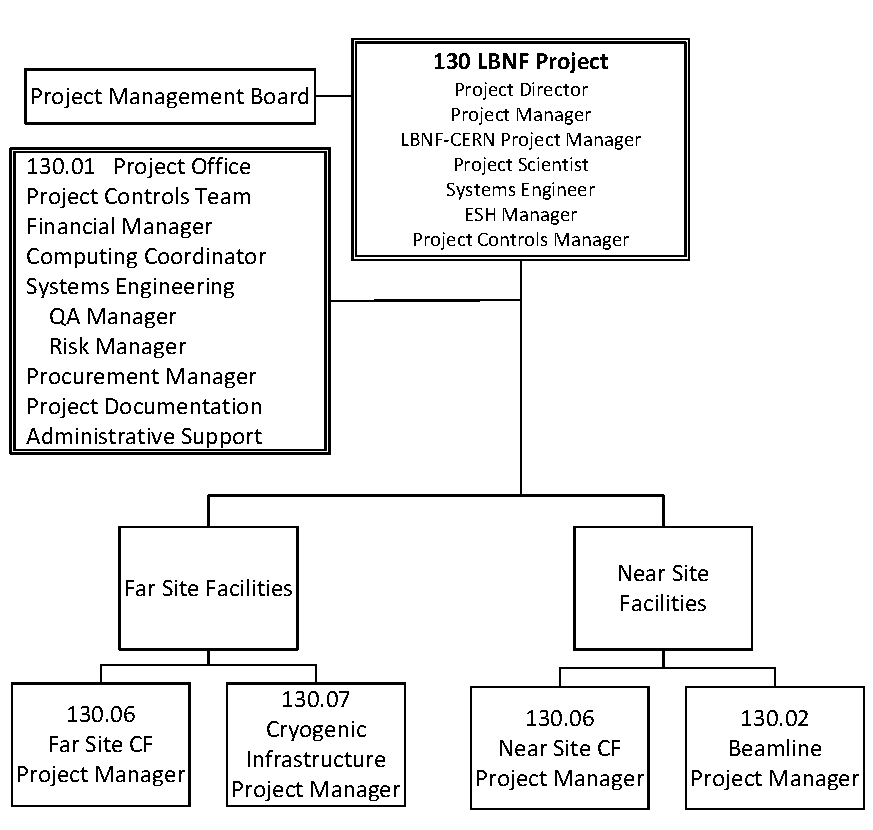
\includegraphics[width=0.8\textwidth]{lbnf-wbs-to-level3}
\end{cdrfigure}

The design and construction of LBNF is supported by other laboratories and consultants/contractors that provide scientific, engineering, and technical expertise. A full description of LBNF Project Management is contained within the LBNF Project Management Plan \fixme{[ref]}.

%%%%%%%%%%%%%%%%%%%%%%%%%%%%%%%
\subsection{Fermilab}  % Eric, it seems weird to have the other two sections without this one.

As the host laboratory for the LBNF Project and the Near Site for the Beamline and DUNE Near Detector, Fermilab provides leadership for the LBNF Project. The LBNF Project organization is headed by the LBNF Project Director who is also the Fermilab Deputy Director for LBNF and reports directly to the Fermilab Director. The Project Director also is the head of the Fermilab Divisions containing the resources needed to execute the Far Site Facilities and Near Site Facilities subprojects.  Any personnel working more than half-time on these subprojects would typically be expected to become a member of one of these divisions, while other contributors will likely be matrixed in part-time roles from other Fermilab Divisions.  The heads of the other Fermilab Divisions work with the L1 and L2 project managers to supply the needed resources on an annual basis.  The management structure described above is currently being transitioned into and will not be fully in place until the Fall of 2015.  


%%%%%%%%%%%%%%%%%%%%%%%%%%%%%%%
\subsection{SDSTA and SURF}

LBNF plans to construct facilities at SURF to house the DUNE far detector. SURF is owned by the state of South Dakota and managed by the South Dakota Science and Technology Authority (SDSTA). \fixme{define SURF, SDSTA earlier}

Current SURF activities include operations necessary for allowing safe access to the 4850L of the mine, which houses the existing and under-development science experiments. The DOE is presently funding SDSTA ongoing operations through Lawrence Berkeley National Laboratory (LBNL) and its SURF Operations Office through FY16; this is expected to change to funding through Fermilab starting in FY17. 

The LBNF Far Site Facilities Manager is also an employee of SDSTA and is contracted to Fermilab to provide management and coordination of the Far Site Conventional Facilities (CF) and Cryogenics Infrastructure subprojects. LBNF contracts directly with SDSTA for the design of the required CF at SURF; whereas the actual construction of the CF will be directly contracted from Fermilab. Coordination between SDSTA and the LBNF Project is necessary to ensure efficient operations at SURF. This will be facilitated via an agreement being developed between SDSTA and Fermilab regarding the LBNF Project \fixme{[new reference]} that defines responsibilities and methods for working jointly on LBNF Project design and construction. A separate agreement will be written for LBNF Operations. 

%%%%%%%%%%%%%%%%%%%%%%%%%%%%%%%
\subsection{CERN}

The European Organization for Nuclear Research (CERN) will participate in the LBNF Project by providing cryogenic facilities and equipment to support the far detectors as well as some technical components required for the neutrino beamline. As a key partner in the Cryogenics Infrastructure subproject, CERN will provide engineering and technical support for the design and production of specific components and coordinate with others in LBNF on the installation of the identified deliverables. CERN engineers and scientists will participate in the LBNF project as assigned managers for the CERN contributions.
Details of the agreements with CERN will be contained in \fixme{[name the agreements here]}.  

CERN and Fermilab are developing a common cryogenics team to design and produce the Cryogenics Infrastructure subproject deliverables for the far site. CERN provides engineers and other staff as needed to complete their agreed-upon deliverables.  

%%%%%%%%%%%%%%%%%%%%%%%%%%%%%%%
\subsection{Coordination within LBNF}

The LBNF WBS defines the scope of the work. All changes to the WBS must be approved by the LBNF Project Manager prior to implementation. At the time of CD-1-Refresh, the LBNF WBS is in transition. Both the current and the post CD-1-R WBS is shown in Figure~\ref{fig:lbnf-wbs} to demonstrate how the scope will map from one WBS to the other. 

LBNF uses internal management boards to coordinate and manage within specific Project areas and across all aspects of the Project.  These boards are described here.


\textbf{Project Management Board:} LBNF uses a Project Management Board to provide formal advice to the Project Director on matters of importance to the LBNF Project as a whole. Such matters include (but are not limited to) those that:
\begin{itemize}
\item have significant technical, cost, or schedule impact on the Project
\item have impacts on more than one L2 subproject
\item affect the management systems for the Project
\item have impacts on or result from changes to other Projects on which LBNF is dependent
\item result from external reviews or reviews called by the Project Director
\end{itemize}
The Management Board serves as the
\begin{itemize}
\item LBNF Change Control Board, as described in the Configuration Management Plan \fixme{[ref]}
\item Risk Management Board, as described in the Fermilab Risk Management Plan  \fixme{[ref]}
\end{itemize}

\textbf{Beamline Technical Board:} The role of the LBNF Beamline Technical Board (TB) is to provide recommendations and advice to the Beamline Project Manager on important technical decisions that affect the design and construction of the Beamline. The members of the Technical Board must have knowledge of the Project objectives and priorities in order to perform this function. The Beamline Project Manager chairs the Beamline TB. The Beamline Project Engineer is the Scientific Secretary of the Board and co-chairs the Beamline TB as needed. 

\textbf{FSCF Neutrino Cavity Advisory Board:} The FSCF Project has engaged three international experts in hard rock underground construction to advise it periodically through the design and construction process regarding excavation at SURF. The board meets at the request of the FSCF-PM, generally on site to discuss specific technical issues. The board produces a report with its findings and conclusions for project information and action. 



%%%%%%%%%%%%%%%%%%%%%%%%%%%%%%%%%%%%%%%%%%%%%%%%%%%%%
\section{DUNE}

%%%%%%%%%%%%%%%%%%%%%%%%%%%%%%
\subsection{DUNE Collaboration Structure}

The DUNE Collaboration brings together the members of the international science community 
interested in participating in the DUNE experiment.  The Collaboration defines the scientific goals of the experiment and subsequently 
the requirements on the experimental facilities needed to achieve these goals.  The Collaboration also provides the scientific effort required for the design and construction of the DUNE detectors, operation of the experiment, and analysis of the 
collected data. There are four main elements in the DUNE organizational structure:  
\begin{itemize}
\item the DUNE Collaboration, composed of the General Assembly of the collaboration and the DUNE Institutional Board (IB)     
\item DUNE Management, composed of the two co-spokespersons, the Technical Coordinator (TC), and the Resource Coordinator (RC), who along
  with the IB chair and five other members of the collaboration form the DUNE Executive Committee (EC)
\item the DUNE Project Office (PO)
\item the DUNE Science Team, including the Physics and Software/Computing coordinators. 
\end{itemize}
The relationships between these entities is illustrated in Figure~\ref{fig:dune-org}.

\begin{cdrfigure}[DUNE Project and Collaboration Organization]{dune-org}{DUNE Project and Collaboration Organization}
  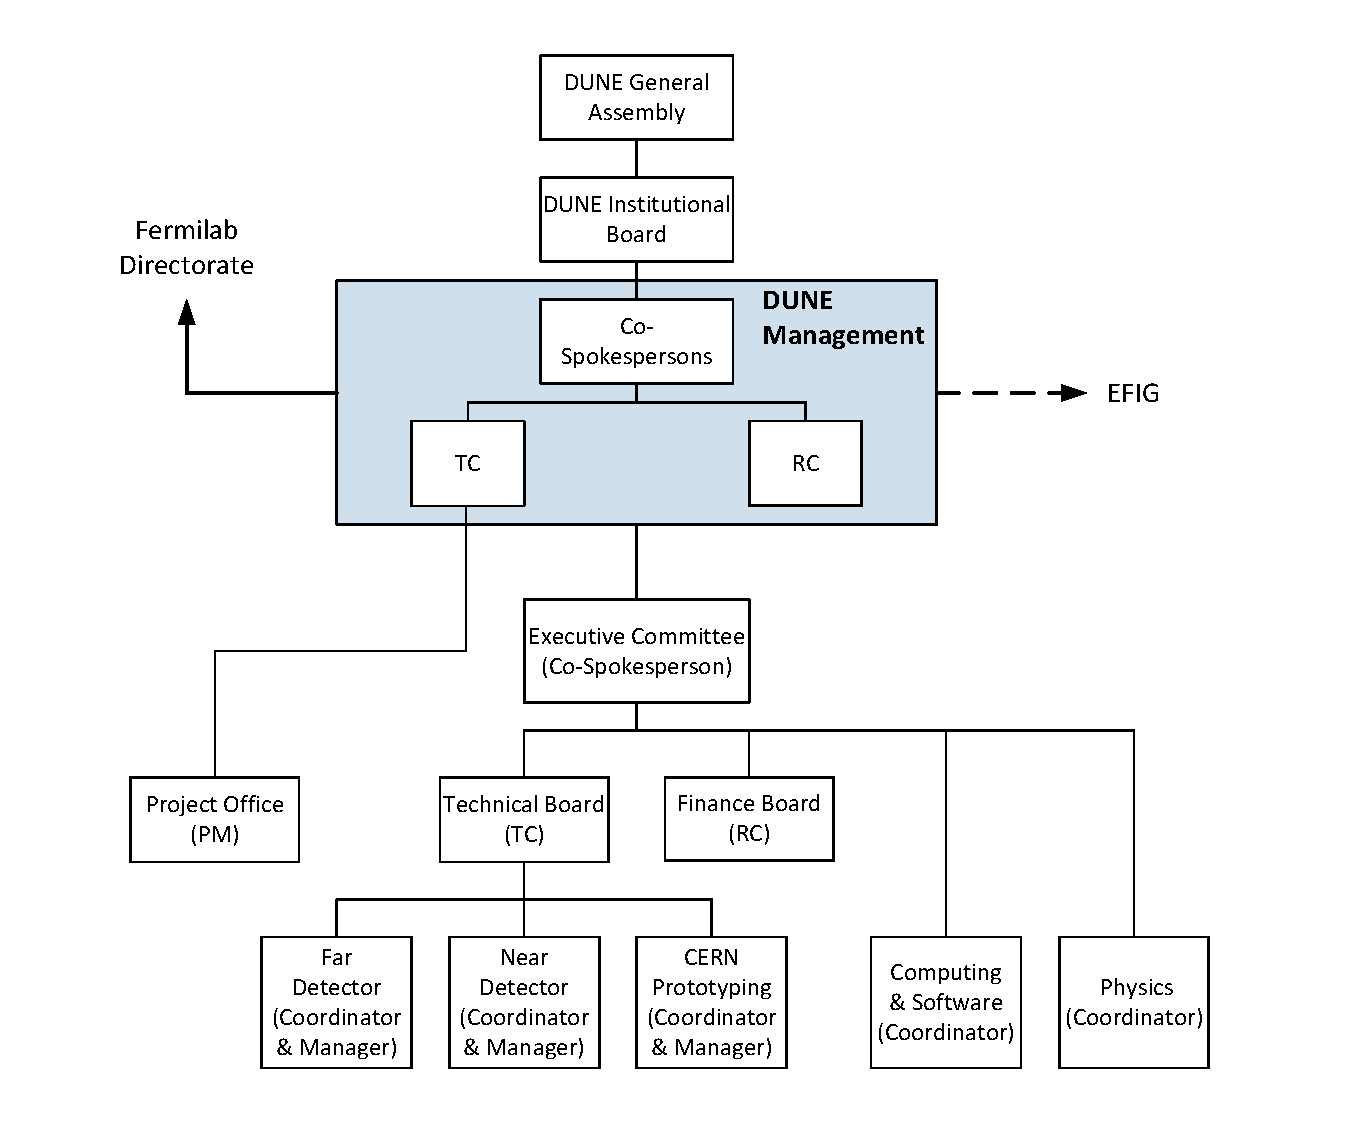
\includegraphics[width=0.95\textwidth]{dune-collaboration-org}
\end{cdrfigure}

\fixme{(for Anne) command to keep figure from floating ...}
\begin{cdrfigure}[DUNE Work Breakdown Structure]{dune-wbs}{DUNE Work Breakdown Structure}
  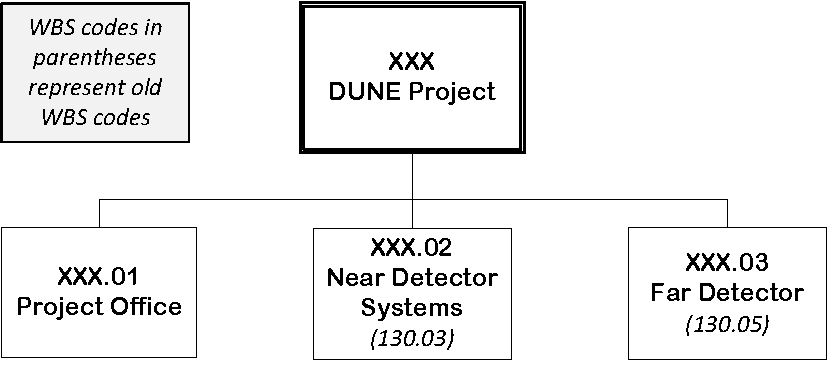
\includegraphics[width=0.8\textwidth]{dune-wbs-to-level3}
\end{cdrfigure}

%%%%%%%%%%%%%%%%%%%%%%%%%%%%%%
\subsection{Responsibilities of the DUNE Leadership}

The main responsibilities of the different roles are summarized below:
\begin{itemize}
  \item \textbf{The DUNE General Assembly} is composed of all members of the collaboration, it is consulted on major strategic decisions 
    through open plenary sessions at collaboration meetings and is informed through regular collaboration phone calls;
  \item \textbf{The DUNE Institutional Board} represents the institutes of the collaboration. It is composed of one representative from each 
    of the member institutions and has responsibility for Collaboration governance.  The IB has final authority over Collaboration 
    membership issues and defines requirements for inclusion of individuals within the DUNE authorship list. The IB is also responsible    
    for establishing and monitoring the process through which the co-spokespeople are selected to serve as leaders of the collaboration.   
  \item \textbf{The DUNE co-spokespersons} are accountable to the collaboration. They 
    are responsible for the day-to-day running of the collaboration and for representing the collaboration to Fermilab, funding 
    agencies, and the broader scientific community.
  \item \textbf{The DUNE Executive Committee (EC)} is chaired by the longest serving co-spokesperson and is the primary 
    decision-making body of the collaboration. Membership of the EC includes the co-spokespeople, DUNE Project Office leaders, IB 
    chair, and five additional Collaboration members (three elected IB representatives and two additional members selected by the co-
    spokespeople). The EC operates by consensus. In cases where consensus cannot be reached, 
    authority lies with the spokespeople. If the co-spokespeople disagree, the TC will arbitrate.
  \item \textbf{The Technical Coordinator (TC)} reports to the spokespersons and the Fermilab director. 
     The TC acts as the project director 
    and is responsible for the implementation of the scientific and technical strategy of the collaboration through the DUNE project office.
    The TC is also responsible for the management of the DOE contributions to the DUNE project.  
     The Technical Coordinator prepares and chairs the meetings of the Technical Board of the experiment collaboration.
     \item \textbf{The Technical Board (TB)} discusses and approves the technical planning for all subsystems of the DUNE detector;
       \item \textbf{The Resource Coordinator (RC)} reports to the spokespersons and the Fermilab director. The RC
    is responsible for coordinating the financial planning and other
resources issues of the collaboration. The RC is responsible in particular for
the management of the common resources of the Collaboration (common fund).
The Resources Coordinator organizes and chairs the meetings of the Finance Board (internal) of
the experiment collaboration. The RC is responsible for the
preparation of the Memoranda of Understanding of the Collaboration.
    \item \textbf{The Finance Board (FB)} is responsible for dealing with matters related to
the costs and resources of the Collaboration, evaluation of the contributions, relations with the
funding agencies and all administrative matters.  
    \item \textbf{The DUNE Science Team} is led by the physics coordinator and the software/computing coordinator and is responsible for the management of the DUNE scientific working groups.
    \item \textbf{The DUNE Project Office (PO)} provides the project management for the design, construction, installation, and commissioning of the DUNE near and far detectors. DUNE will be run as an international project matching DOE requirements. This implies maintaining a full cost and schedule for the entire project, from which the DOE-funded portion can be extracted and monitored in a manner that satisfies DOE reporting requirements. The DUNE Project Office will have direct control over DOE project funds and any common fund collected from the U.S. and international stakeholders. International contributions to the DUNE project will be in the form of deliverables as defined in formal Memoranda of Understanding (MOU). These contributions will be tracked through detailed sub-project milestones. The entire Project (including international contributions) will be subject to the DOE critical decision process incorporating a CD-2 approval of its baseline cost and schedule and a CD-3 approval for moving forward with construction.  The high-level WBS structure of the Project is illustrated in Figure~\ref{fig:dune-wbs}.
    \item \textbf{DUNE Technical Working Groups} The organization of the technical working groups of the DUNE collaboration is the responsibility of the L2 managers in the DUNE project.
\end{itemize}


%%%%%%%%%%%%%%%%%%%%%%%%%%%%%%%%%%%%%%%%%%%%%%%%%%%%%
\section{LBNF/DUNE Advisory and Coordinating Structures}
\label{sec:lbnf-dune-interface}

The LBNF and DUNE projects are overseen by a number of advisory and coordinating bodies as shown in Figure~\ref{fig:lbnfdune-org}.  The role of the different bodies are described in the following sections.  

\begin{cdrfigure}[LBNF/DUNE Project Structure]{lbnfdune-org}{LBNF/DUNE Project Structure}
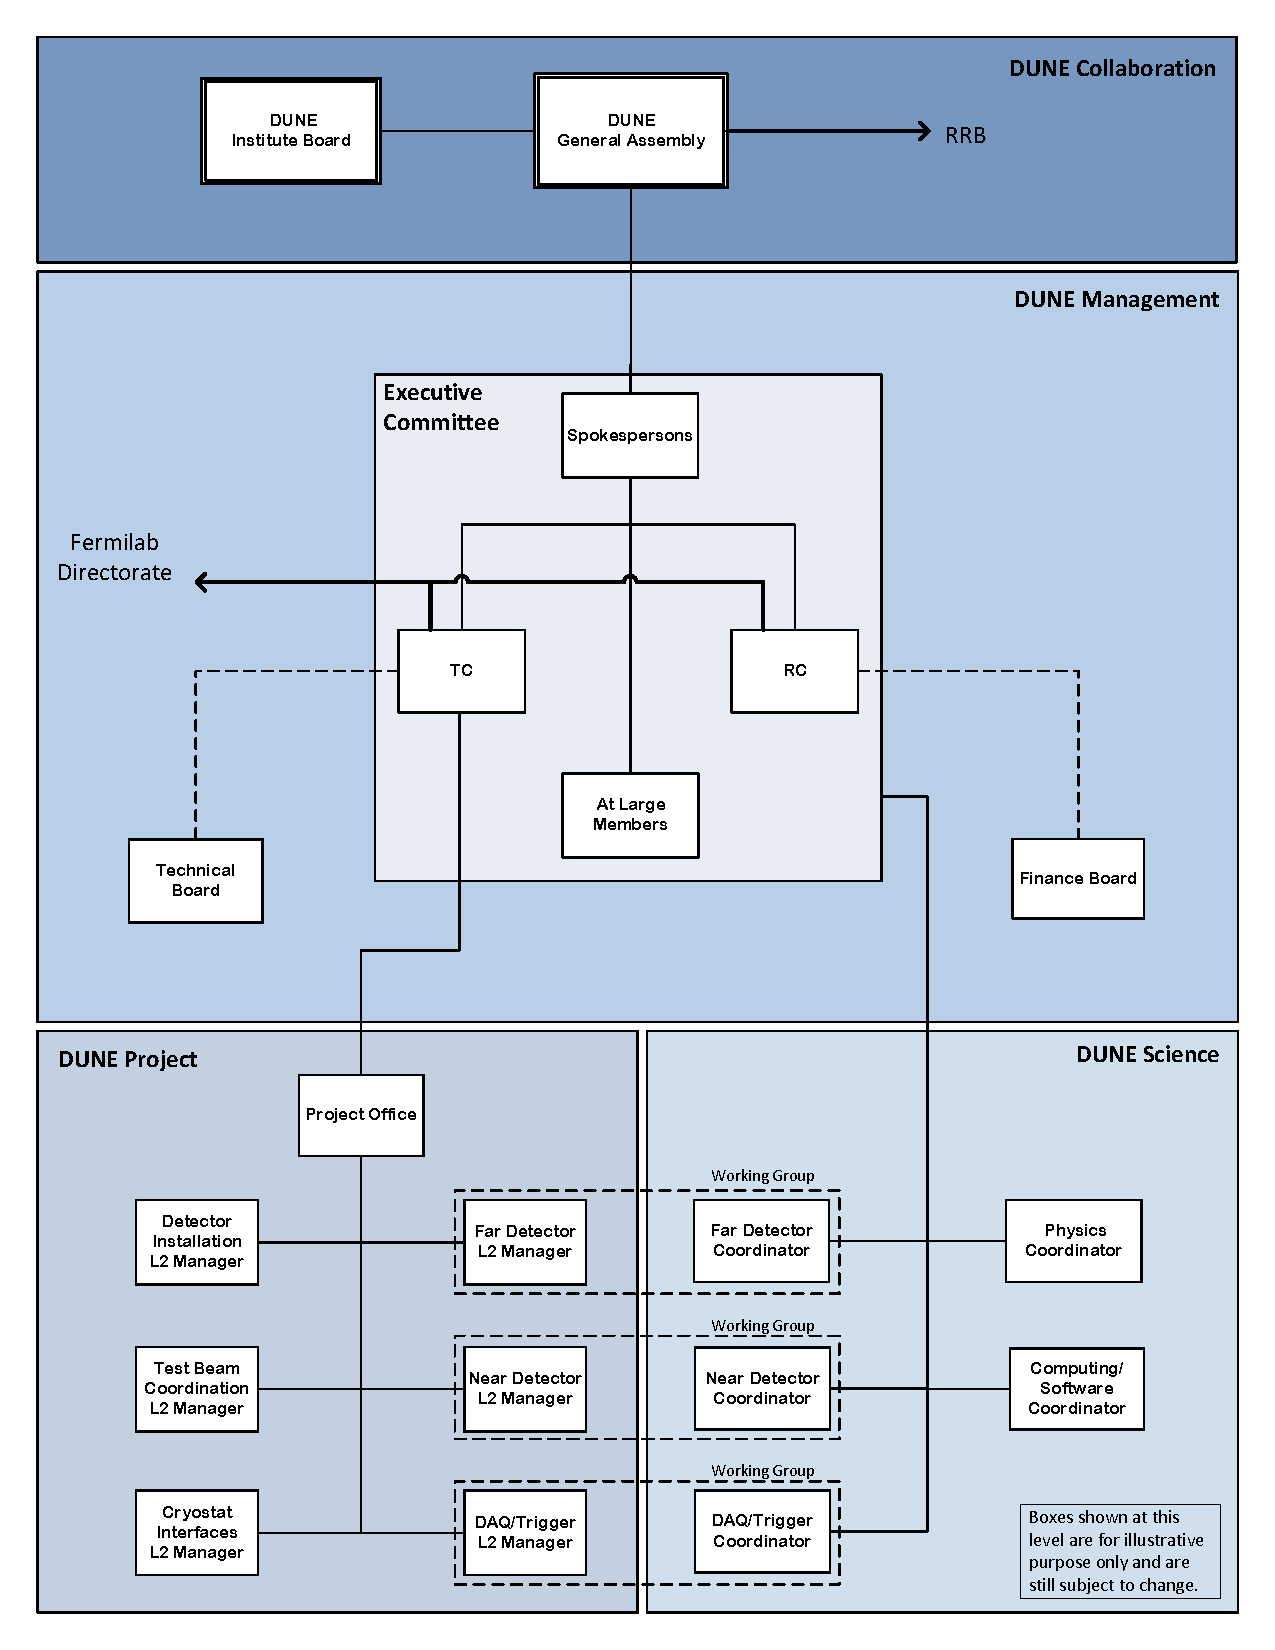
\includegraphics[width=0.8\textwidth]{lbnf-dune-structure}
\end{cdrfigure}

\subsection{International Advisory Committee (IAC) }

The International Advisory Committee (IAC) provides primary oversight and coordination of the two projects.  This group is made up representatives from each of the funding agencies involved in the program and provides global coordination across the entire enterprise.  In particular, this group is responsible for developing a plan that divides the financial responsibilities for constructing the facilities and detectors.   This group also has a leading role in developing the bi-lateral and subsidiary agreements between the DOE and other international stakeholders required to advance the program. 

\subsection{Fermilab, the Host Laboratory}

As the host laboratory, Fermilab has a direct responsibility for the design, construction, commissioning, and operation of the facilities and infrastructure that support the program.  In this capacity, Fermilab reports directly to the    DOE through the Fermilab Site Office (FSO).   Fermilab also has an important oversight role for the DUNE project itself as well as an important coordination role in ensuring that interface issues between the two projects are completely understood. 

\subsection{LBNC Advisory Committee}

	The LBNC is an international, external advisory committee tasked with providing peer review for the two projects.  This group monitors the projects through regular meetings with the management teams and provides guidance   to the Fermilab director in his oversight role.  The Fermilab director appoints the head of this committee, who is then responsible for appointing additional committee members. \fixme{The LBNC Advisory Committee body needs to be distinguished better from the IAC; e.g., if the IAC is more about funding, is this more about science?}

\subsection{Resource Research Board (RRB)}

 	This body serves as the operational arm of the International Advisory Committee.  The Fermilab Director in coordination with the DUNE RC defines its membership, which includes representatives of the funding agencies contributing to the projects.  The deputy lab director is the chair of the board and organizes regular meetings to ensure that the needed  flow of funding to the projects is maintained.  The RRB is charged with defining different national contributions to the projects and the associated Memoranda of Understanding.   It is also responsible for understanding in-kind contributions to common projects. 

\subsection{Experiment-Facility Interface Group (EFIG)}

	The EFIG is the official body tasked with coordinating the LBNF and DUNE projects.  The Fermilab director controls the membership of this group, and his deputy serves as its head.  Group membership includes members of the Fermilab management such as the Chief Project Officer, members of the LBNF project management team, the DUNE co-spokespeople, as well as the DUNE Technical and Resource Coordinators.  The director at his discretion appoints additional members to ensure fulfillment of the group functions, which are to oversee and ensure the required coordination of the LBNF and DUNE projects during the design, construction, and operational phases of the program.    
	
\subsection{DUNE Collaboration}	

	The collaboration, in consultation with the Fermilab Director, is responsible for forming the international project team responsible for designing and constructing the detectors.  The Technical Coordinator (TC) and Resource Coordinator (RC) serve as the lead managers of this international project team and are selected jointly by the spokespeople and the Fermilab director.  Because the international project incorporates contributions from a number of different funding agencies, the international DUNE project is responsible for satisfying individual tracking and reporting requirements associated with each of the different contributions.


